\documentclass[11pt]{article}
\usepackage[margin=1in]{geometry}
\usepackage[T1]{fontenc}
\usepackage{lmodern,microtype,amsmath,amssymb,amsthm,booktabs,graphicx}
\usepackage{xcolor,enumitem}
\usepackage[colorlinks=true,linkcolor=blue!45!black,citecolor=blue!45!black,urlcolor=blue!45!black]{hyperref}
\setlist{itemsep=2pt,topsep=4pt}
\newtheorem{proposition}{Proposition}
\newtheorem{corollary}{Corollary}
\newcommand{\Sc}{\mathcal S}
\newcommand{\Pa}{\mathcal P}
\title{Buying warning-delay tolerance\\with fixed mine escape routes}
\author{}
\date{Working preprint --- October 25, 2026}
\begin{document}
\maketitle
\begin{abstract}
A regional flood alarm may tell a miner which part of a mine is affected without identifying the exact inrush point or how long flooding has been underway. We study an evacuation plan that remains implementable with that information: one route, fixed in advance for each worker location and alarm region, followed immediately upon receipt. The question is how much extra distance is required to guarantee escape across specified source scenarios and notification delays. Under first-in--first-out tunnel travel and permanent closures, a target delay reduces to a common-route feasibility problem at one departure time. We solve it by multi-scenario label search and distinguish lack of a common route from physical infeasibility even with perfect source information. In an exploratory volume-transfer model, an exhaustive node-source study of one competition-network region raises the number of outside-region origins supporting a 30-minute delay from 268 of 548 on the baseline shortest routes to 501 with a 20\% distance allowance, and 545 without a distance limit. A separate two-network screen shows why source coverage matters: improvements on design sources can disappear or reverse on unseen sources. These are finite-scenario, model-relative guarantees, not calibrated mine-safety predictions. The results support evaluating fixed evacuation plans by the delay they can withstand and the distance that guarantee costs, while making their information and hazard assumptions explicit.
\end{abstract}

\section{Introduction}
An emergency route map is useful only if the person reading it has enough information to choose the prescribed route. An instruction that requires the exact flood source or the true onset time may be unavailable when an alarm reaches an underground worker. A simpler instruction is conceivable: ``for an alarm from the eastern region, take this marked route.'' Such a route must cope with several possible water sources and with water that has already been spreading before notification.

Mine water inrush is a sudden entry of water into underground workings, for example from a water-bearing formation or flooded void. Connected roadways provide both escape paths and channels for the water. Flooding can slow movement and eventually make passages impassable. A shortest route on a dry map can therefore be fragile even when a slightly longer alternative remains usable.

Existing mine-inrush research computes earliest-arrival paths in evolving water conditions \cite{wu2020}. Sensor-location research addresses how rapidly an inrush can be detected, explicitly allowing water to spread before reaching a monitor \cite{wu2021}. Between detection and dynamic routing lies a practical planning question:
\begin{quote}
Given only a regional alarm, can a worker follow a route fixed before the accident and still escape after a specified notification delay? How much detour is needed to obtain that guarantee?
\end{quote}
The route may depend on the worker's starting location and the reported region. It may not depend on the unreported exact source, the unknown event age, or future observations. The worker leaves immediately after receiving the alarm.

We formulate a guarantee-first problem: for a target delay, find a common feasible route across the source scenarios, then minimize distance within that feasible set. This order matters. A 5\% detour allowance is an experimental comparison, not a presumed operational requirement. We also compute feasibility without a distance limit and report the resulting burden.

The central empirical finding is that fixed regional routes can substantially outperform dry shortest routes within the stated model, but their apparent robustness depends strongly on which sources are included. For one region, all 113 candidate source nodes are evaluated against all 548 eligible outside-region origins. A 20\% allowance increases the number supporting a 30-minute delay from 268 to 501. Yet a route designed using eight sources and successful on another eight supports only about 1.5 minutes when a missed source is added. Thus a convincing plan needs both a route and an explicit account of the hazards against which it was checked.

Our contribution is a decision formulation, an auditable finite-scenario computation, and an investigation of this coverage problem. The underlying tools---FIFO path propagation, resource dominance, and robust scenario constraints---are established optimization ideas. We do not claim a new general shortest-path algorithm or the first use of robust routing. Preparing several policies and selecting one after information arrives is studied in \(K\)-adaptability \cite{hanasusanto}; here we deliberately specify the smaller information set available at the alarm. Section~\ref{sec:time} also explains why a menu indexed only by delay does not increase the maximum guaranteed delay under our assumptions.

This study grew out of a mine-inrush modeling competition \cite{cumcm}. It uses a competition network and a network extracted from a CAD drawing, but does not assume the reader has seen either the competition solution or the extraction files. The flood calculation is an uncalibrated volume-transfer surrogate. The numerical results establish properties of specified hazard schedules, not the effectiveness of a real mine's emergency plan.

\section{What the alarm reveals}
\subsection{Three timestamps, not one}
Let \(t_0\) denote physical inrush onset, \(t_{\rm det}\) detection, and \(t_{\rm rec}\) receipt of the alarm by the worker. If immediate departure follows receipt, the relevant event age is
\[
 d=t_{\rm rec}-t_0
   =(t_{\rm det}-t_0)+(t_{\rm rec}-t_{\rm det}).
\]
Any additional response time can be included in \(d\). A recorded detection timestamp can help identify the second term, provided it is communicated and clocks are comparable. It does not by itself identify the first term. Water may take time to reach a sensor; the sensor-placement study of Wu et al.~\cite{wu2021} explicitly models detection within a prescribed time after inrush. Conversely, a witnessed event or a sufficiently informative monitoring system might constrain onset closely. We do not assume that every mine knows, or that every mine fails to know, the true delay.

Our base information model supplies a region \(R\) and an assurance that departure occurs no later than a planning horizon \(\tau\) after onset. The worker need not know the realized \(d\). The planner asks whether the prescribed route works for \emph{every} \(0\le d\le\tau\). This is a design specification, not an instruction to wait after receiving an alarm.

Warnings based on precursor risk before an inrush are a different information process. They are not modeled by simply assigning a negative notification delay. Likewise, the region reported by a sensor need not coincide with the physical source region. We assume the alarm's source-region interpretation is correct; uncertain classification would require enlarging the scenario set.

\subsection{The scenario set is part of the claim}
For a reported region \(R\), let \(\Sc_R\) be the specified set of possible hazard scenarios. A scenario may contain a source location, flow history, hydraulic parameters, and their resulting tunnel conditions. The main experiments vary source location while holding the other parameters fixed; a later sensitivity changes inflow.

No probability distribution over accidents is inferred from a list of nodes. A statement that a route works in all sampled scenarios is a finite-set guarantee. It becomes a guarantee over a physical region only if the set or an accompanying bound adequately represents that region. In particular, checking every graph node does not check every location along every tunnel.

A route assignment is written \(P(v,R)\), where \(v\) is a worker origin. It is chosen offline. During an incident, the observed region selects the assignment, and the worker follows it without receiving the exact source. This is the mathematical version of a region-indexed emergency route map. We do not study how such a map should be designed or tested with users.

\section{Delay guarantees and the price of a detour}
Let \(G=(V,A)\) be a directed representation of the tunnel network, with positive arc lengths \(\ell_a\), an origin \(v\), and a set \(X\) of escape endpoints. Both directions of a tunnel may appear as arcs. For scenario \(s\), let \(A_a^s(t)\) be the arrival time at the end of arc \(a\) when entering at time \(t\). Set it to \(+\infty\) when that traversal is infeasible.

We assume these extended arrival functions are nondecreasing: entering later cannot produce an earlier feasible arrival. This is the first-in--first-out (FIFO) property. Closures are permanent, and traversing a path earlier cannot make an otherwise feasible traversal fail. These assumptions hold for the piecewise-speed, permanent-closure schedules used below; they need not hold for arbitrary receding-water models.

For a path \(P=(a_1,\ldots,a_m)\), compose the arc functions to obtain its arrival \(A_P^s(d)\). Its deadline is
\[
 D_s(P)=\sup\{d\ge0:A_P^s(d)<\infty\},
\]
with \(D_s(P)=-\infty\) if it cannot be traversed even at onset. Our implementation also stores backward-computed algebraic deadlines below zero to diagnose this case; such values are not safe departure times.

Define the common deadline and length by
\[
 D_R(P)=\min_{s\in\Sc_R}D_s(P),\qquad
 L(P)=\sum_{a\in P}\ell_a.
\]
A route for a regional alarm is evaluated against all the scenarios before taking the minimum. Choosing a different path after seeing each true source would answer a different, better-informed problem.

\begin{proposition}[Endpoint reduction]\label{prop:endpoint}
Fix a finite scenario set and a path whose scenario-wise feasible departure sets are downward closed and include their finite endpoints. For \(\tau\ge0\), the path is feasible under every scenario for every departure \(d\in[0,\tau]\) if and only if it is feasible under every scenario at \(d=\tau\).
\end{proposition}
\begin{proof}
Necessity follows by selecting the endpoint. For sufficiency, downward closure in each scenario gives feasibility for every earlier departure; intersecting the scenario-wise statements proves the claim.
\end{proof}
The endpoint convention holds for the schedules below. With strict physical thresholds, one can instead certify a slightly smaller departure time. This elementary reduction prevents a continuous interval of delays from becoming an unnecessary second simulation grid.

For a desired delay \(\tau\), define
\begin{equation}
 L_R^*(v,\tau)=\min\{L(P):P\text{ joins }v\text{ to }X,
                     \ A_P^s(\tau)<\infty\ \forall s\in\Sc_R\}.
 \label{eq:target}
\end{equation}
The value is \(+\infty\) if no common route exists. Let \(L_0(v)\) be the dry shortest distance to an escape endpoint. The relative detour needed for the guarantee is
\[
 \rho_R(v,\tau)=L_R^*(v,\tau)/L_0(v)-1.
\]
We exclude exit nodes, where \(L_0=0\). Equation~\eqref{eq:target} prioritizes feasibility and uses distance only to select an economical feasible plan.

The complementary budget question is
\begin{equation}
 D_R^*(v,\varepsilon)=\max_{P:L(P)\le(1+\varepsilon)L_0(v)}D_R(P).
 \label{eq:budget}
\end{equation}
A target \(\tau\) is attainable with budget \(\varepsilon\) exactly when \(\rho_R(v,\tau)\le\varepsilon\). More distance cannot decrease the design-set optimum, but it need not improve performance on an omitted source.

\subsection{When knowing the delay helps}\label{sec:time}
Suppose the source set remains \(\Sc_R\), the path constraints do not change with the reported delay, and the objective is to guarantee escape for every delay up to \(\tau\).

\begin{corollary}[Delay-only menus do not extend the guarantee]\label{cor:menu}
Under Proposition~\ref{prop:endpoint}, allowing a worker to select among finitely many precomputed routes using the exact delay does not make a target \(\tau\) feasible if no single common route can achieve it.
\end{corollary}
\begin{proof}
The route selected at \(\tau\) must work for all sources in \(\Sc_R\). By Proposition~\ref{prop:endpoint}, that same route works at all earlier delays. It is therefore a valid single-route plan for the whole interval.
\end{proof}
The corollary also holds under a common length cap. Delay information can still reduce walking burden: an early alarm may justify a shorter route while a late alarm requires a detour. With an estimated age interval \([d_-,d_+]\), a route safe at \(d_+\) covers that interval under the same assumptions. Two or three age bands could approximate this distance benefit.

The conclusion changes if observations also narrow the possible sources, or if feasibility is not downward closed. More informative sensor observations may eliminate scenarios and genuinely enlarge the feasible set. We therefore keep delay-indexed menus outside the main model rather than introduce additional policies without establishing what information selects them.

\subsection{Separating physical impossibility from insufficient information}
For each scenario, let \(U_s(v)\) be the latest departure when the path may be selected knowing \(s\). Then
\begin{equation}
 D_R(P)\le \min_{s\in\Sc_R}U_s(v)
 \quad\text{for every fixed }P.                         \label{eq:upper}
\end{equation}
If the right side is below \(\tau\), at least one scenario is impossible even with perfect source information. If every \(U_s(v)\ge\tau\), yet \eqref{eq:target} is infeasible, the obstruction is different: separately feasible scenarios require incompatible route choices. Finally, a common route may exist but exceed a prescribed length budget. These three failures should not be merged into a single ``no improvement'' category.

\section{Computation and verification}
\subsection{A common-path label search}
At a fixed target \(\tau\), a label at node \(u\) records traveled length \(l\) and the vector of scenario arrival times
\[
 (l,t_1,\ldots,t_k),\qquad k=|\Sc_R|.
\]
The origin label is \((0,\tau,\ldots,\tau)\). Extending along arc \(a\) adds \(\ell_a\) and replaces every \(t_s\) by \(A_a^s(t_s)\). If any component is infeasible, the extension is rejected. This creates one shared node sequence, not one independent path per scenario.

At the same node, a label dominates another if it has no larger length and no later arrival in every scenario. FIFO ensures that any feasible suffix of the dominated label is also feasible from the dominating label. We retain all nondominated labels without an approximate dominance tolerance or label-count cap. A dry shortest-distance lower bound orders the queue and prunes extensions exceeding a length cap. Scenario-specific reverse deadlines \(U_s\) prune labels that cannot reach an exit in some scenario.

The first exit extracted by the length-based search gives \(L_R^*\). A path containing a cycle cannot improve the optimum: removing the cycle shortens it and reaches the following node no later in every scenario. The finite graph therefore admits a simple optimal path whenever a feasible path exists. Label sets can nevertheless grow exponentially; this is not a claim of polynomial complexity. Each query has a three-second execution limit, and a limit would be reported as unresolved rather than infeasible. No reported production query timed out.

To solve \eqref{eq:budget}, we bisect the departure target, using \eqref{eq:upper} as an upper bound. The main screen caps the objective at 3,600 seconds and stops when the bracket width is below 0.5 seconds. Direct target-guarantee experiments do not need bisection. One illustrative budget curve is also computed without the one-hour cap.

\subsection{Checks on the algorithm and returned routes}
We tested the multi-scenario search on 100 independently generated six-node graphs with three hazard scenarios each. Exhaustive enumeration of every simple path supplied the reference. All 400 fixed-departure feasibility and minimum-length comparisons agreed; all 100 optimized-deadline brackets contained the enumerated optimum. These tests check the new common-route implementation, not the validity of flood predictions.

Returned routes are checked against their length budgets and scenario-wise deadlines. In the dense-source experiment, the guarantee is recomputed from the full stored node sequence for all 113 sources. Source identities, paths, solver statuses, lower and upper deadline brackets, and model inputs are retained. Unknown outcomes are not converted into successes or failures.

\section{Networks, hazard schedules, and experiment design}
\subsection{Two networks and illustrative alarm regions}
The competition network has 664 nodes, 978 undirected tunnels, and two escape endpoints after insertion of the supplied reference source location. The CAD-derived network has 1,592 nodes, 2,084 tunnels, and four designated shaft-bottom endpoints. Widths are 4 and approximately 4.99 meters, respectively. A shaft-bottom endpoint terminates our route calculation; reaching the surface is not simulated.

The CAD graph was extracted using geometric snapping, intersection splitting, and shaft connectors. Roof elevations serve as a proxy for relative floor elevations under a constant-height assumption. Those choices require engineering validation. The competition graph is also a model input, not a surveyed accident reconstruction.

For each network, median \(x\) and \(y\) coordinates define four geographic quadrants. These illustrate coarse source-region alarms. They are not asserted to be actual sensor sectors, geologically equiprobable source areas, or operational boundaries. Candidate sources exclude escape endpoints and the auxiliary reference source node. Worker-source coincidence is excluded in the selected screen; the dense experiment considers workers outside its entire source region.

\subsection{The flood surrogate and its limits}
The inherited event-driven model accounts for inflow volume on the tunnel graph. Water is split among available level or downhill outlets; uphill outlets become active when those choices are unavailable. Covered tunnels transmit water or store it according to a propagation tree, and saturated branches cause backing up. A tunnel's depth proxy is stored volume divided by width and length. Stored volume never decreases.

The base source supplies \(0.5\,\mathrm{m^3\,s^{-1}}\), with a nominal 3-meter tunnel height. A passage becomes wet at its modeled first-entry time and closes permanently at mean depth 0.3 meters. This threshold is a modeling convention, not a universal human-safety limit. Travel speed changes from dry to wet; movement with and against the assigned flow can differ. For a tunnel of length \(L\), wetting time \(w\), and closure \(b\), arrival is calculated exactly by traversing the dry portion at \(v_d\) and the remaining distance at \(v_w\), then checking arrival by \(b\). All experiments use \(v_d\ge v_w>0\), giving FIFO behavior.

The initial two-network screen retains the competition speeds \(4/2/1\,\mathrm{m\,s^{-1}}\) for dry travel, movement with the flow, and movement against it, respectively. Because the dry speed is high for sustained evacuation, the principal dense-source and all-origin experiments use \(1.3/0.7/0.5\,\mathrm{m\,s^{-1}}\). These are sensitivity values, not fitted pedestrian laws.

Volume-accounting residuals are checked, but conservation does not establish realistic flood arrival. The model omits resolved momentum, spatial depth profiles, junction losses, pumping, debris, velocity-dependent stability, and human congestion. Its propagation-tree and event-order conventions can matter. No hydraulic calibration is claimed for either network. We therefore interpret the results as a route-planning study conditional on hazard schedules.

\subsection{Discovery, source coverage, and broader checks}
The experiment has three stages, which must not be mistaken for independent replications.
\begin{enumerate}
\item \textbf{Two-network screen.} In each of eight network-region combinations, a fixed random seed selects eight design sources and eight distinct held-out sources. All eligible origins are screened on the design scenarios. Up to 12 whose baseline route has a deadline between zero and one hour, plus up to four with an initially infeasible baseline, are randomly selected per region. This gives 123 origin-region pairs: 96 baseline-feasible and 27 initially infeasible. Budgets are 0, 5, 10, and 20\%, later extended to 50, 100\%, and no cap.
\item \textbf{Dense-source investigation.} A promising competition-network case, origin P0104 with a southeast alarm, is selected after viewing the screen. All 113 eligible source nodes in that quadrant are simulated. The original route is checked and then redesigned against the complete node set. Twenty-four randomly selected tunnel-midpoint sources are subsequently tested against the fixed redesigned route, without retraining it.
\item \textbf{All-origin target study.} Holding that 113-source set fixed, all 548 eligible origins outside the quadrant are evaluated at 10-, 20-, and 30-minute delay targets using the slower speeds. This removes the favorable-origin selection within this one region, but does not establish prevalence across regions or mines.
\end{enumerate}
The initial protocol and source identities were recorded before those runs. Dense-source checks and the all-origin study are adaptive follow-ups, not a preregistered external confirmation. Node counts describe designed cases; they are not probabilities of surviving an accident.

\section{Results}
\subsection{Many origins benefit when a target guarantee comes first}
Table~\ref{tab:targets} gives the principal all-origin result. For each target, each origin receives its own fixed route, common to all 113 sources. The optimized route can differ across target specifications, but cannot change with the realized source within a specification.

\begin{table}[htbp]\centering
\caption{Origins supporting each delay target, out of 548 outside-region origins. The source set contains all 113 candidate nodes in the southeast quadrant.}\label{tab:targets}
\begin{tabular}{lrrr}\toprule
Distance allowance & 10 min & 20 min & 30 min\\\midrule
Baseline dry shortest route &292&278&268\\
At most 5\% extra &424&403&403\\
At most 10\% extra &498&457&435\\
At most 20\% extra &520&509&501\\
At most 50\% extra &529&523&518\\
At most 100\% extra &533&527&526\\
No distance cap &547&546&545\\\bottomrule
\end{tabular}
\end{table}

At 30 minutes, the 20\% allowance supports 233 additional origins relative to the baseline. Removing the cap supports 277 additional origins. Thus the benefit is not confined to the illustrative worker location. Nevertheless, these origins share a network, exits, a source set, and a flood model; they are spatially correlated comparisons rather than hundreds of independent accidents.

The uncapped result does not mean all routes are operationally acceptable. At the 30-minute target, some common routes are about 15.11 kilometers long, and the largest relative detour is approximately 408\%. The calculation establishes modeled traversability, not the ability of a particular worker to sustain that journey.

Three origins still fail at 30 minutes without a distance cap. For one, a scenario-specific reverse deadline is already below the target: even perfect source information cannot provide escape in that scenario. For two, each source separately admits escape, but no single path works for the entire source set. This is the distinction in \eqref{eq:upper}: a failure of regional fixed-route information is different from a failure of physical escape options.

\begin{figure}[htbp]\centering
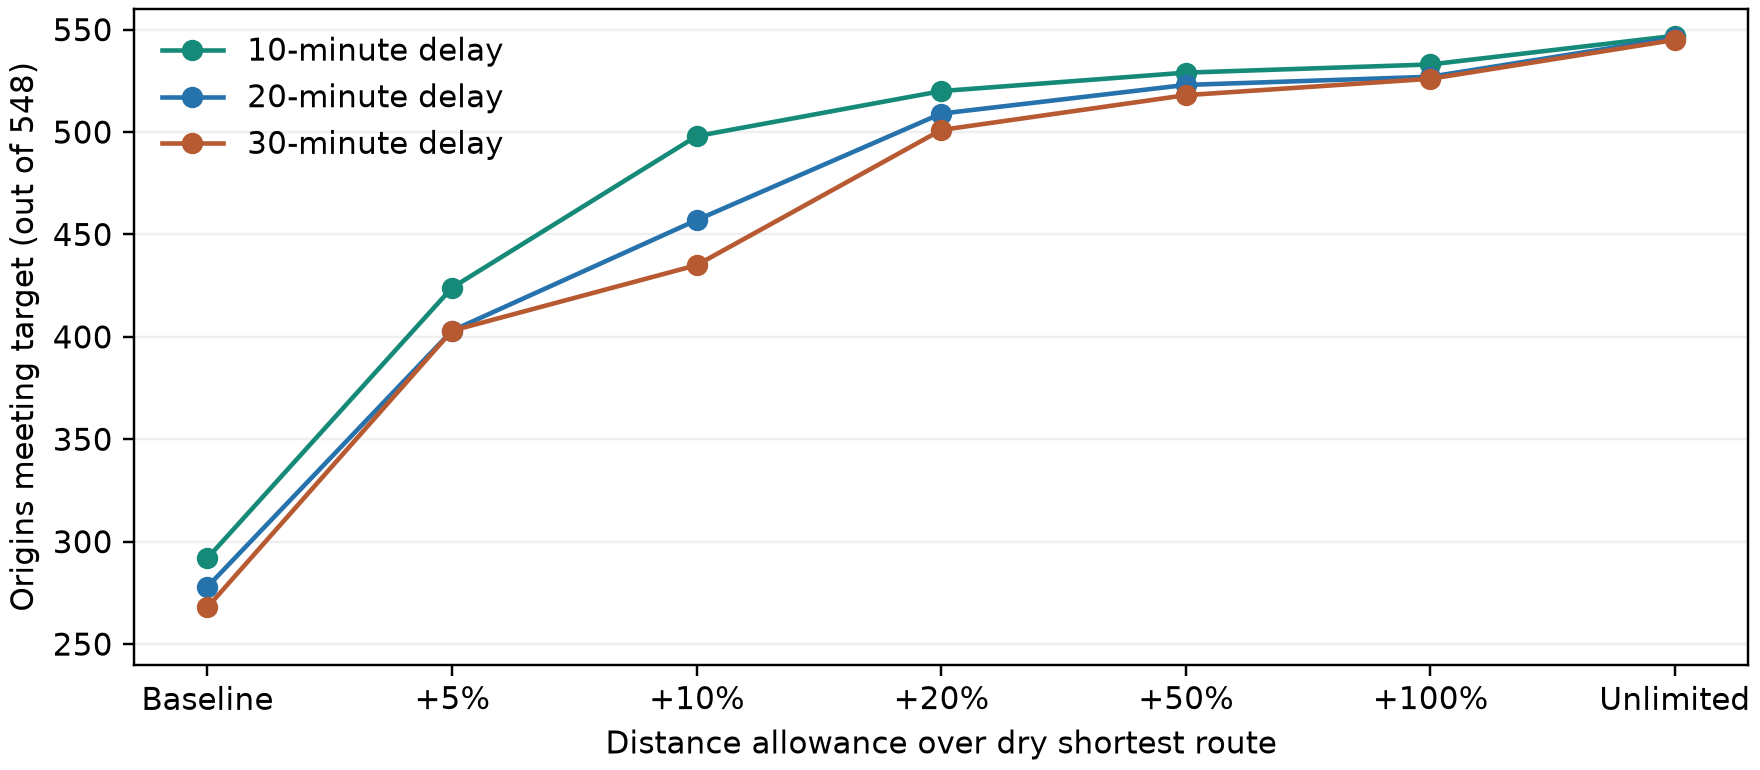
\includegraphics[width=.87\linewidth]{figures/target_counts.png}
\caption{Distance budgets buy additional target guarantees, with diminishing gains in this region. ``Unlimited'' removes the length constraint, not the flood constraints.}\label{fig:targets}
\end{figure}

\subsection{A representative route and a non-smooth trade-off}
For P0104, the dry shortest route is 2,701.36 meters. Across the dense source set, that route fails even at onset in some scenarios. A common route of 2,768.58 meters---67.23 meters, or 2.49\%, longer---has deadline 11.94 minutes at the slower speeds. With the competition speeds, the same route supports 16.47 minutes.

The benefit is not a smooth reward for every extra meter. Allowing 20\% yields a 3,240.94-meter route and an 80.16-minute common deadline under the slower speeds. Budgets of 50 and 100\% return the same optimum. With no distance limit, the optimum reaches 360.17 minutes, but requires a 17.21-kilometer route. Those values were computed without the one-hour optimization cap and bracketed to less than 0.5 seconds; the long-time flood predictions remain particularly model dependent.

The 24 new midpoint sources do not reduce the 11.94-minute guarantee of the 2,768.58-meter route. Their worst deadline exceeds 68 minutes at the slower speeds. This is useful stress evidence against a purely node-specific success, but it does not establish coverage of every interior point. Nor were all routes in Table~\ref{tab:targets} tested against these midpoint sources.

\subsection{Eight successful test sources can miss a damaging source}
The dense case also provides a warning about evaluation. Using eight design sources at the competition speeds, the originally selected route supported the one-hour design horizon. It also supported that horizon for all eight held-out sources. Yet a further source, P0172, reduced its deadline to 89.88 seconds. Holding the route fixed while expanding source coverage exposed the failure; changing paths separately for each test source would have concealed it.

Reoptimization across all 113 nodes changes a local branch from P0174--P0631--P0171 to P0174--P0172--P0171. The branches have nearly equal length, but different worst-source deadlines. The redesigned route reaches the 16.47-minute common deadline at the competition speeds. Figure~\ref{fig:coverage} shows the full source-wise comparison, including failures of the original shortest route.

\begin{figure}[htbp]\centering
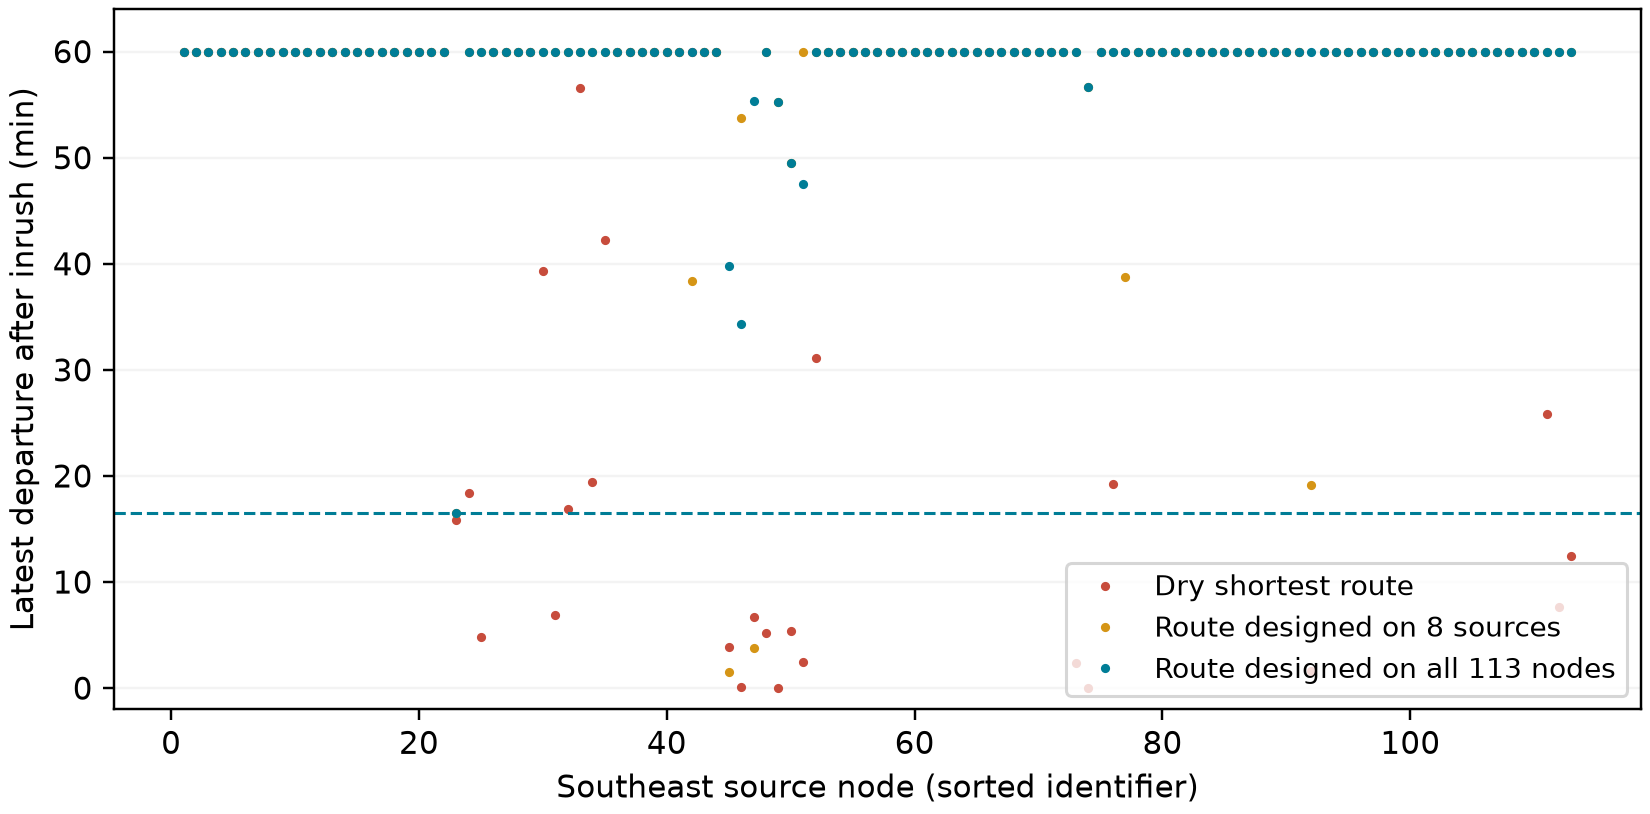
\includegraphics[width=\linewidth]{figures/source_coverage.png}
\caption{All 113 source nodes for worker P0104, using the original competition speeds. Values below zero or above 60 minutes are clipped for display.}\label{fig:coverage}
\end{figure}

This example was selected after the screen. It demonstrates a failure mode of sparse source coverage, not an estimated probability that a new source will invalidate a plan. The subsequent exhaustive node study repairs that particular omission within the finite candidate set; it does not validate the hydraulic model.

\subsection{The two-network screen is less favorable on unseen sources}
For the 48 baseline-feasible selected pairs in each network, Table~\ref{tab:heldout} counts changes of at least one minute in worst-source deadline, clipped to the interval from zero to one hour. Each route is designed on eight sources, then evaluated unchanged on eight different sources from the same quadrant.

\begin{table}[htbp]\centering
\caption{Counts out of 48 selected baseline-feasible pairs per network. The 27 additional initially infeasible pairs remain in the archived results.}\label{tab:heldout}
\begin{tabular}{llrrr}\toprule
Network & Budget & Design gain & Held-out gain & Held-out loss\\\midrule
Competition &5\%&38&14&4\\
Competition &20\%&40&14&4\\
Competition &Uncapped&41&14&7\\
CAD-derived &5\%&37&4&6\\
CAD-derived &20\%&46&9&6\\
CAD-derived &Uncapped&47&10&6\\\bottomrule
\end{tabular}
\end{table}

A larger route set improves the design optimum, but does not guarantee better held-out behavior. In the competition screen, uncapped optimization increases the count of held-out losses. This is not paradoxical: optimization protects the included sources and has no constraint for omitted ones. Also, some held-out baselines are already above one hour, leaving no room for improvement in the clipped metric. The table is a stress-test summary, not a learning-curve estimate or a comparison between statistically independent mines.

\subsection{Fixed-route sensitivity to flow and event ordering}\label{sec:sensitivity}
To separate plan sensitivity from the benefit of reoptimization, we retained the 545 uncapped routes that meet the 30-minute target in the dense-source study and evaluated the same routes under altered schedules. Their speeds remain \(1.3/0.7/0.5\,\mathrm{m\,s^{-1}}\).

For this constant-inflow volume-transfer model, multiplying inflow by a factor rescales event times inversely; this homogeneity was separately checked on recomputed flows in the original model audit. Applying it to \(Q=0.25,0.5,1.0\,\mathrm{m^3\,s^{-1}}\), all 545 routes retain the target at the first two flows, but only 329 retain it at the doubled flow. This is an internal model sensitivity, not evidence that real flood dynamics scale uniformly with inflow.

We also reran all 113 source simulations with the model's alternative ordering of simultaneous edge events. All 545 fixed routes retained the 30-minute guarantee under that convention. This check rules out a failure under the tested ordering change; it does not validate the propagation-tree physics or establish invariance to arbitrary junction models.

The flow result is consequential: a source-location guarantee at one prescribed inflow does not silently extend to unknown inflow magnitude. A practical scenario set would need to include such uncertainty explicitly. The current headline counts should retain their fixed-flow qualifier.

\section{Interpretation and limitations}
The main result concerns how to evaluate an implementable plan. Regional information can support a common route that accepts more distance in exchange for a specified delay guarantee. The all-origin study shows a substantial improvement over dry shortest routes in one modeled region. The held-out and dense-source comparisons show that the guarantee is only as broad as its hazard set.

Knowing the event age has a narrower role than it might first appear. Under downward-closed feasibility, a route that survives the latest admissible notification also survives earlier notifications. Delay-only route menus can save walking distance for early alarms, but cannot extend the worst-case guarantee while the source set and constraints remain unchanged. If future observations reduce the possible sources, adaptive routing can have a different value. A sensor-informed extension should model the observation process rather than grant the routing method access to the true simulated source.

Four limitations prevent direct deployment conclusions.
\begin{enumerate}
\item \textbf{Hydraulic credibility.} The schedules come from a volume-transfer surrogate, not a calibrated transient hydraulic solver. Average tunnel depth, propagation-tree junctions, permanent closure, and uncertain geometry may alter which branch is preferable. More routing experiments cannot cure that limitation.
\item \textbf{Coverage and selection.} Dense node coverage is available for one region; the rest of the two-network experiment uses small source samples. The dense case was selected adaptively, and the all-origin population excludes the source region. Interior sources, multiple simultaneous inrushes, uncertain alarm classification, and general flow histories remain outside the guarantee.
\item \textbf{Human and exit assumptions.} Speed is prescribed without fatigue, group interaction, visibility, or stability modeling. Long routes may be unacceptable. Reaching a designated network exit is treated as completion; ascent and refuge operations are not modeled.
\item \textbf{Monotone time structure.} Endpoint reduction and the delay-menu corollary require downward-closed path feasibility. Receding hazards, temporary barriers, waiting in refuges, or non-FIFO conditions may require an interval-wide treatment and can give time information additional value.
\end{enumerate}

The numerical precision of a deadline bracket should not be confused with physical accuracy. Seconds in the solver output document optimization consistency; they do not warrant second-level evacuation instructions. Similarly, improvement counts quantify this graph experiment rather than an accident survival probability.

\section{Conclusion}
A regional evacuation plan can be evaluated by a concrete requirement: one route must remain feasible for every included source when the alarm arrives as late as a specified time. In the studied hazard schedules, useful guarantees often require modest detours, while some origins need much longer routes or cannot share a feasible route across scenarios at all.

The next research priority is to preserve this information-constrained question while replacing uncertain schedules with better-supported ones. Which local branches determine the common deadline under a transient hydraulic model? How densely must source locations be represented before the guarantee stabilizes? Can sensor observations distinguish the scenarios that demand incompatible routes? These questions connect the route map to the information and physical evidence needed to justify it.

\appendix
\section{Reproducibility and provenance}
The accompanying package preserves the earlier studies separately. The current evidence is in \texttt{regional\_escape/}; the manuscript and figures are in \texttt{regional\_alarm\_paper/}. Principal scripts are:
\begin{itemize}
\item \texttt{prepare.py}: geographic regions, fixed source lists, and source-wise flood schedules.
\item \texttt{study.py}, \texttt{test\_solver.py}: common-route labels, budget search, and exhaustive small-graph checks.
\item \texttt{dense.py}, \texttt{dense\_optimize.py}: full southeast node-source evaluation and redesign.
\item \texttt{target\_guarantees.py}: all 548 outside-region origins at three delay targets.
\item \texttt{midpoint\_check.py}, \texttt{paper\_sensitivity.py}: interior-source and fixed-route model sensitivities.
\item \texttt{longer\_detours.py}, \texttt{uncapped\_example.py}: larger budgets and the uncapped illustrative optimum.
\end{itemize}
The initial protocol, source design files, complete route sequences, numerical brackets, and failure statuses are retained in JSON. The code uses Python with NetworkX, NumPy, pandas, openpyxl, Shapely, and Matplotlib; the accompanying README gives commands and environment notes. Flood preparation must finish before route evaluation begins. Cached results must not be reused after changing a protocol without a new output directory.

\begin{samepage}
This study was developed with AI assistance and requires human authorship review before external circulation. New work must not be attributed retrospectively to the original competition submission.
\end{samepage}

\begin{thebibliography}{9}\small
\bibitem{wu2020}
Q. Wu et al. Finding the earliest arrival path through a time-varying network for evacuation planning of mine water inrush. \emph{Safety Science} 130 (2020), 104836.
\href{https://doi.org/10.1016/j.ssci.2020.104836}{doi:10.1016/j.ssci.2020.104836}.
\bibitem{wu2021}
Q. Wu, Z. Du, Y. Zhao, H. Xu, and X. Zhang. Optimal location of water level sensors for monitoring mine water inrush based on the set covering model. \emph{Scientific Reports} 11 (2021), 2621.
\href{https://doi.org/10.1038/s41598-021-82121-7}{doi:10.1038/s41598-021-82121-7}.
\bibitem{hanasusanto}
G. A. Hanasusanto, D. Kuhn, and W. Wiesemann. \emph{K-Adaptability in Two-Stage Robust Binary Programming}. Author manuscript, Optimization Online.
\url{https://optimization-online.org/wp-content/uploads/2014/03/4294.pdf}.
\bibitem{cumcm}
China Society for Industrial and Applied Mathematics. \emph{CUMCM 2025, Problem D: Mine water-inrush propagation and escape planning}. Supplied problem statement and attachments. Competition information: \url{https://en.mcm.edu.cn/}.
\end{thebibliography}
\end{document}
